% Options for packages loaded elsewhere
\PassOptionsToPackage{unicode}{hyperref}
\PassOptionsToPackage{hyphens}{url}
%
\documentclass[
]{article}
\usepackage{amsmath,amssymb}
\usepackage{lmodern}
\usepackage{iftex}
\ifPDFTeX
  \usepackage[T1]{fontenc}
  \usepackage[utf8]{inputenc}
  \usepackage{textcomp} % provide euro and other symbols
\else % if luatex or xetex
  \usepackage{unicode-math}
  \defaultfontfeatures{Scale=MatchLowercase}
  \defaultfontfeatures[\rmfamily]{Ligatures=TeX,Scale=1}
\fi
% Use upquote if available, for straight quotes in verbatim environments
\IfFileExists{upquote.sty}{\usepackage{upquote}}{}
\IfFileExists{microtype.sty}{% use microtype if available
  \usepackage[]{microtype}
  \UseMicrotypeSet[protrusion]{basicmath} % disable protrusion for tt fonts
}{}
\makeatletter
\@ifundefined{KOMAClassName}{% if non-KOMA class
  \IfFileExists{parskip.sty}{%
    \usepackage{parskip}
  }{% else
    \setlength{\parindent}{0pt}
    \setlength{\parskip}{6pt plus 2pt minus 1pt}}
}{% if KOMA class
  \KOMAoptions{parskip=half}}
\makeatother
\usepackage{xcolor}
\usepackage[margin=1in]{geometry}
\usepackage{color}
\usepackage{fancyvrb}
\newcommand{\VerbBar}{|}
\newcommand{\VERB}{\Verb[commandchars=\\\{\}]}
\DefineVerbatimEnvironment{Highlighting}{Verbatim}{commandchars=\\\{\}}
% Add ',fontsize=\small' for more characters per line
\usepackage{framed}
\definecolor{shadecolor}{RGB}{248,248,248}
\newenvironment{Shaded}{\begin{snugshade}}{\end{snugshade}}
\newcommand{\AlertTok}[1]{\textcolor[rgb]{0.94,0.16,0.16}{#1}}
\newcommand{\AnnotationTok}[1]{\textcolor[rgb]{0.56,0.35,0.01}{\textbf{\textit{#1}}}}
\newcommand{\AttributeTok}[1]{\textcolor[rgb]{0.77,0.63,0.00}{#1}}
\newcommand{\BaseNTok}[1]{\textcolor[rgb]{0.00,0.00,0.81}{#1}}
\newcommand{\BuiltInTok}[1]{#1}
\newcommand{\CharTok}[1]{\textcolor[rgb]{0.31,0.60,0.02}{#1}}
\newcommand{\CommentTok}[1]{\textcolor[rgb]{0.56,0.35,0.01}{\textit{#1}}}
\newcommand{\CommentVarTok}[1]{\textcolor[rgb]{0.56,0.35,0.01}{\textbf{\textit{#1}}}}
\newcommand{\ConstantTok}[1]{\textcolor[rgb]{0.00,0.00,0.00}{#1}}
\newcommand{\ControlFlowTok}[1]{\textcolor[rgb]{0.13,0.29,0.53}{\textbf{#1}}}
\newcommand{\DataTypeTok}[1]{\textcolor[rgb]{0.13,0.29,0.53}{#1}}
\newcommand{\DecValTok}[1]{\textcolor[rgb]{0.00,0.00,0.81}{#1}}
\newcommand{\DocumentationTok}[1]{\textcolor[rgb]{0.56,0.35,0.01}{\textbf{\textit{#1}}}}
\newcommand{\ErrorTok}[1]{\textcolor[rgb]{0.64,0.00,0.00}{\textbf{#1}}}
\newcommand{\ExtensionTok}[1]{#1}
\newcommand{\FloatTok}[1]{\textcolor[rgb]{0.00,0.00,0.81}{#1}}
\newcommand{\FunctionTok}[1]{\textcolor[rgb]{0.00,0.00,0.00}{#1}}
\newcommand{\ImportTok}[1]{#1}
\newcommand{\InformationTok}[1]{\textcolor[rgb]{0.56,0.35,0.01}{\textbf{\textit{#1}}}}
\newcommand{\KeywordTok}[1]{\textcolor[rgb]{0.13,0.29,0.53}{\textbf{#1}}}
\newcommand{\NormalTok}[1]{#1}
\newcommand{\OperatorTok}[1]{\textcolor[rgb]{0.81,0.36,0.00}{\textbf{#1}}}
\newcommand{\OtherTok}[1]{\textcolor[rgb]{0.56,0.35,0.01}{#1}}
\newcommand{\PreprocessorTok}[1]{\textcolor[rgb]{0.56,0.35,0.01}{\textit{#1}}}
\newcommand{\RegionMarkerTok}[1]{#1}
\newcommand{\SpecialCharTok}[1]{\textcolor[rgb]{0.00,0.00,0.00}{#1}}
\newcommand{\SpecialStringTok}[1]{\textcolor[rgb]{0.31,0.60,0.02}{#1}}
\newcommand{\StringTok}[1]{\textcolor[rgb]{0.31,0.60,0.02}{#1}}
\newcommand{\VariableTok}[1]{\textcolor[rgb]{0.00,0.00,0.00}{#1}}
\newcommand{\VerbatimStringTok}[1]{\textcolor[rgb]{0.31,0.60,0.02}{#1}}
\newcommand{\WarningTok}[1]{\textcolor[rgb]{0.56,0.35,0.01}{\textbf{\textit{#1}}}}
\usepackage{graphicx}
\makeatletter
\def\maxwidth{\ifdim\Gin@nat@width>\linewidth\linewidth\else\Gin@nat@width\fi}
\def\maxheight{\ifdim\Gin@nat@height>\textheight\textheight\else\Gin@nat@height\fi}
\makeatother
% Scale images if necessary, so that they will not overflow the page
% margins by default, and it is still possible to overwrite the defaults
% using explicit options in \includegraphics[width, height, ...]{}
\setkeys{Gin}{width=\maxwidth,height=\maxheight,keepaspectratio}
% Set default figure placement to htbp
\makeatletter
\def\fps@figure{htbp}
\makeatother
\setlength{\emergencystretch}{3em} % prevent overfull lines
\providecommand{\tightlist}{%
  \setlength{\itemsep}{0pt}\setlength{\parskip}{0pt}}
\setcounter{secnumdepth}{-\maxdimen} % remove section numbering
\ifLuaTeX
  \usepackage{selnolig}  % disable illegal ligatures
\fi
\IfFileExists{bookmark.sty}{\usepackage{bookmark}}{\usepackage{hyperref}}
\IfFileExists{xurl.sty}{\usepackage{xurl}}{} % add URL line breaks if available
\urlstyle{same} % disable monospaced font for URLs
\hypersetup{
  pdftitle={Project 8 Template},
  hidelinks,
  pdfcreator={LaTeX via pandoc}}

\title{Project 8 Template}
\author{}
\date{\vspace{-2.5em}}

\begin{document}
\maketitle

\begin{Shaded}
\begin{Highlighting}[]
\CommentTok{\# Add to this package list for additional SL algorithms}
\NormalTok{pacman}\SpecialCharTok{::}\FunctionTok{p\_load}\NormalTok{(}
\NormalTok{  tidyverse,}
\NormalTok{  ggthemes,}
\NormalTok{  ltmle,}
\NormalTok{  tmle,}
\NormalTok{  SuperLearner,}
\NormalTok{  tidymodels,}
\NormalTok{  caret,}
\NormalTok{  dagitty,}
\NormalTok{  ggdag,}
\NormalTok{  here)}

\NormalTok{heart\_disease }\OtherTok{\textless{}{-}} \FunctionTok{read\_csv}\NormalTok{(}\StringTok{\textquotesingle{}/Users/alexadia/Documents/GitHub/Computational{-}Social{-}Science{-}Projects/Project 8/heart\_disease\_tmle.csv\textquotesingle{}}\NormalTok{)}
\end{Highlighting}
\end{Shaded}

\begin{verbatim}
## Rows: 10000 Columns: 14
## -- Column specification --------------------------------------------------------
## Delimiter: ","
## dbl (14): age, sex_at_birth, simplified_race, college_educ, income_thousands...
## 
## i Use `spec()` to retrieve the full column specification for this data.
## i Specify the column types or set `show_col_types = FALSE` to quiet this message.
\end{verbatim}

\hypertarget{introduction}{%
\section{Introduction}\label{introduction}}

Heart disease is the leading cause of death in the United States, and
treating it properly is an important public health goal. However, it is
a complex disease with several different risk factors and potential
treatments. Physicians typically recommend changes in diet, increased
exercise, and/or medication to treat symptoms, but it is difficult to
determine how effective any one of these factors is in treating the
disease. In this project, you will explore SuperLearner, Targeted
Maximum Likelihood Estimation (TMLE), and Longitudinal Targeted Maximum
Likelihood Estimation (LTMLE). Using a simulated dataset, you will
explore whether taking blood pressure medication reduces mortality risk.

\hypertarget{data}{%
\section{Data}\label{data}}

This dataset was simulated using R (so it does not come from a previous
study or other data source). It contains several variables:

\begin{itemize}
    \item \textbf{blood\_pressure\_medication}: Treatment indicator for whether the individual took blood pressure medication (0 for control, 1 for treatment)
    \item \textbf{mortality}: Outcome indicator for whether the individual passed away from complications of heart disease (0 for no, 1 for yes)
    \item \textbf{age}: Age at time 1
    \item \textbf{sex\_at\_birth}: Sex assigned at birth (0 female, 1 male)
    \item \textbf{simplified\_race}: Simplified racial category. (1: White/Caucasian, 2: Black/African American, 3: Latinx, 4: Asian American, \newline 5: Mixed Race/Other)
    \item \textbf{income\_thousands}: Household income in thousands of dollars
    \item \textbf{college\_educ}: Indicator for college education (0 for no, 1 for yes)
    \item \textbf{bmi}: Body mass index (BMI)
    \item \textbf{chol}: Cholesterol level
    \item \textbf{blood\_pressure}: Systolic blood pressure 
    \item \textbf{bmi\_2}: BMI measured at time 2
    \item \textbf{chol\_2}: Cholesterol measured at time 2
    \item \textbf{blood\_pressure\_2}: BP measured at time 2
    \item \textbf{blood\_pressure\_medication\_2}: Whether the person took treatment at time period 2 
\end{itemize}

For the ``SuperLearner'' and ``TMLE'' portions, you can ignore any
variable that ends in ``\_2'', we will reintroduce these for LTMLE.

\hypertarget{superlearner}{%
\section{SuperLearner}\label{superlearner}}

\hypertarget{modeling}{%
\subsection{Modeling}\label{modeling}}

Fit a SuperLearner model to estimate the probability of someone dying
from complications of heart disease, conditional on treatment and the
relevant covariates. Do the following:

\begin{enumerate}
    \item Choose a library of at least 5 machine learning algorithms to evaluate. \textbf{Note}: We did not cover how to hyperparameter tune constituent algorithms within SuperLearner in lab, but you are free to do so if you like (though not required to for this exercise). 
    \item Split your data into train and test sets.
    \item Train SuperLearner
    \item Report the risk and coefficient associated with each model, and the performance of the discrete winner and SuperLearner ensemble
    \item Create a confusion matrix and report your overall accuracy, recall, and precision
\end{enumerate}

\begin{Shaded}
\begin{Highlighting}[]
\CommentTok{\# Fit SuperLearner Model}

\DocumentationTok{\#\# sl lib}
\FunctionTok{listWrappers}\NormalTok{()}
\end{Highlighting}
\end{Shaded}

\begin{verbatim}
## All prediction algorithm wrappers in SuperLearner:
\end{verbatim}

\begin{verbatim}
##  [1] "SL.bartMachine"      "SL.bayesglm"         "SL.biglasso"        
##  [4] "SL.caret"            "SL.caret.rpart"      "SL.cforest"         
##  [7] "SL.earth"            "SL.extraTrees"       "SL.gam"             
## [10] "SL.gbm"              "SL.glm"              "SL.glm.interaction" 
## [13] "SL.glmnet"           "SL.ipredbagg"        "SL.kernelKnn"       
## [16] "SL.knn"              "SL.ksvm"             "SL.lda"             
## [19] "SL.leekasso"         "SL.lm"               "SL.loess"           
## [22] "SL.logreg"           "SL.mean"             "SL.nnet"            
## [25] "SL.nnls"             "SL.polymars"         "SL.qda"             
## [28] "SL.randomForest"     "SL.ranger"           "SL.ridge"           
## [31] "SL.rpart"            "SL.rpartPrune"       "SL.speedglm"        
## [34] "SL.speedlm"          "SL.step"             "SL.step.forward"    
## [37] "SL.step.interaction" "SL.stepAIC"          "SL.svm"             
## [40] "SL.template"         "SL.xgboost"
\end{verbatim}

\begin{verbatim}
## 
## All screening algorithm wrappers in SuperLearner:
\end{verbatim}

\begin{verbatim}
## [1] "All"
## [1] "screen.corP"           "screen.corRank"        "screen.glmnet"        
## [4] "screen.randomForest"   "screen.SIS"            "screen.template"      
## [7] "screen.ttest"          "write.screen.template"
\end{verbatim}

\begin{Shaded}
\begin{Highlighting}[]
\NormalTok{library}\OtherTok{\textless{}{-}}\FunctionTok{c}\NormalTok{(}\StringTok{\textquotesingle{}SL.mean\textquotesingle{}}\NormalTok{, }\StringTok{\textquotesingle{}SL.glmnet\textquotesingle{}}\NormalTok{, }\StringTok{\textquotesingle{}SL.earth\textquotesingle{}}\NormalTok{, }\StringTok{"SL.lm"}\NormalTok{, }\StringTok{"SL.nnet"}\NormalTok{) }\CommentTok{\#picked these arbitrarily}

\DocumentationTok{\#\# Train/Test split}
\CommentTok{\# need to kick the variables that start with 2 since we ignore for this section}
\NormalTok{heart\_disease\_no2}\OtherTok{\textless{}{-}}\NormalTok{heart\_disease}\SpecialCharTok{\%\textgreater{}\%}\FunctionTok{select}\NormalTok{(}\SpecialCharTok{{-}}\NormalTok{bmi\_2, }\SpecialCharTok{{-}}\NormalTok{chol\_2, }\SpecialCharTok{{-}}\NormalTok{blood\_pressure\_2, }\SpecialCharTok{{-}}\NormalTok{blood\_pressure\_medication\_2)}
\CommentTok{\#now get split}
\FunctionTok{set.seed}\NormalTok{(}\DecValTok{24}\NormalTok{)}
\NormalTok{heart\_disease\_split}\OtherTok{\textless{}{-}}\FunctionTok{initial\_split}\NormalTok{(heart\_disease\_no2)}
\CommentTok{\# Declare the training set with rsample::training()}
\NormalTok{train }\OtherTok{\textless{}{-}} \FunctionTok{training}\NormalTok{(heart\_disease\_split)}

\CommentTok{\# set training}
\NormalTok{y\_train }\OtherTok{\textless{}{-}}\NormalTok{ train }\SpecialCharTok{\%\textgreater{}\%} 
  \FunctionTok{pull}\NormalTok{(mortality) }

\NormalTok{x\_train }\OtherTok{\textless{}{-}}\NormalTok{ train }\SpecialCharTok{\%\textgreater{}\%}
  \FunctionTok{select}\NormalTok{(}\SpecialCharTok{{-}}\NormalTok{mortality)}

\CommentTok{\# Do the same procedure with the test set}
\NormalTok{test }\OtherTok{\textless{}{-}} \FunctionTok{testing}\NormalTok{(heart\_disease\_split)}

\NormalTok{y\_test }\OtherTok{\textless{}{-}}\NormalTok{ test }\SpecialCharTok{\%\textgreater{}\%}
  \FunctionTok{pull}\NormalTok{(mortality)}

\NormalTok{x\_test }\OtherTok{\textless{}{-}}\NormalTok{ test }\SpecialCharTok{\%\textgreater{}\%}
  \FunctionTok{select}\NormalTok{(}\SpecialCharTok{{-}}\NormalTok{mortality)}

\DocumentationTok{\#\# Train SuperLearner}
\NormalTok{sl\_q1}\OtherTok{\textless{}{-}} \FunctionTok{SuperLearner}\NormalTok{(}\AttributeTok{Y =}\NormalTok{ y\_train,}
                         \AttributeTok{X =}\NormalTok{ x\_train,}
                         \AttributeTok{family =} \FunctionTok{binomial}\NormalTok{(),}
                         \AttributeTok{SL.library =}\NormalTok{ library)}
\end{Highlighting}
\end{Shaded}

\begin{verbatim}
## Loading required namespace: earth
\end{verbatim}

\begin{Shaded}
\begin{Highlighting}[]
\DocumentationTok{\#\# Risk and Coefficient of each model}
\NormalTok{sl\_q1}
\end{Highlighting}
\end{Shaded}

\begin{verbatim}
## 
## Call:  
## SuperLearner(Y = y_train, X = x_train, family = binomial(), SL.library = library) 
## 
## 
## 
##                    Risk      Coef
## SL.mean_All   0.2498864 0.0000000
## SL.glmnet_All 0.2364546 0.0000000
## SL.earth_All  0.2300872 0.8484226
## SL.lm_All     0.2361808 0.1515774
## SL.nnet_All   0.2504166 0.0000000
\end{verbatim}

\begin{Shaded}
\begin{Highlighting}[]
\DocumentationTok{\#\# Discrete winner and superlearner ensemble performance}

\DocumentationTok{\#\# Confusion Matrix}

\NormalTok{preds }\OtherTok{\textless{}{-}} \FunctionTok{predict}\NormalTok{(sl\_q1,}
\NormalTok{                 x\_test,}
                 \AttributeTok{onlySL =} \ConstantTok{TRUE}\NormalTok{)}

\CommentTok{\# start with y\_test}
\NormalTok{validation }\OtherTok{\textless{}{-}}\NormalTok{ y\_test }\SpecialCharTok{\%\textgreater{}\%}
  \CommentTok{\# add our predictions}
  \FunctionTok{bind\_cols}\NormalTok{(preds}\SpecialCharTok{$}\NormalTok{pred[,}\DecValTok{1}\NormalTok{]) }\SpecialCharTok{\%\textgreater{}\%}
  \CommentTok{\# rename columns}
  \FunctionTok{rename}\NormalTok{(}\AttributeTok{obs =} \StringTok{\textasciigrave{}}\AttributeTok{...1}\StringTok{\textasciigrave{}}\NormalTok{,}
         \AttributeTok{pred =} \StringTok{\textasciigrave{}}\AttributeTok{...2}\StringTok{\textasciigrave{}}\NormalTok{) }\SpecialCharTok{\%\textgreater{}\%}
  \FunctionTok{mutate}\NormalTok{(}\AttributeTok{pred =} \FunctionTok{ifelse}\NormalTok{(pred }\SpecialCharTok{\textgreater{}=}\NormalTok{ .}\DecValTok{5}\NormalTok{, }
                           \DecValTok{1}\NormalTok{,}
                           \DecValTok{0}\NormalTok{))}
\end{Highlighting}
\end{Shaded}

\begin{verbatim}
## New names:
## * `` -> `...1`
## * `` -> `...2`
\end{verbatim}

\begin{Shaded}
\begin{Highlighting}[]
\FunctionTok{head}\NormalTok{(validation)}
\end{Highlighting}
\end{Shaded}

\begin{verbatim}
## # A tibble: 6 x 2
##     obs  pred
##   <dbl> <dbl>
## 1     1     1
## 2     0     1
## 3     0     1
## 4     1     1
## 5     0     1
## 6     0     1
\end{verbatim}

\begin{Shaded}
\begin{Highlighting}[]
\NormalTok{caret}\SpecialCharTok{::}\FunctionTok{confusionMatrix}\NormalTok{(}\FunctionTok{as.factor}\NormalTok{(validation}\SpecialCharTok{$}\NormalTok{pred),}
                       \FunctionTok{as.factor}\NormalTok{(validation}\SpecialCharTok{$}\NormalTok{obs))}
\end{Highlighting}
\end{Shaded}

\begin{verbatim}
## Confusion Matrix and Statistics
## 
##           Reference
## Prediction    0    1
##          0  257   66
##          1  920 1257
##                                           
##                Accuracy : 0.6056          
##                  95% CI : (0.5861, 0.6248)
##     No Information Rate : 0.5292          
##     P-Value [Acc > NIR] : 8.566e-15       
##                                           
##                   Kappa : 0.1755          
##                                           
##  Mcnemar's Test P-Value : < 2.2e-16       
##                                           
##             Sensitivity : 0.2184          
##             Specificity : 0.9501          
##          Pos Pred Value : 0.7957          
##          Neg Pred Value : 0.5774          
##              Prevalence : 0.4708          
##          Detection Rate : 0.1028          
##    Detection Prevalence : 0.1292          
##       Balanced Accuracy : 0.5842          
##                                           
##        'Positive' Class : 0               
## 
\end{verbatim}

\hypertarget{discussion-questions}{%
\subsection{Discussion Questions}\label{discussion-questions}}

\begin{enumerate}
    \item Why should we, in general, prefer the SuperLearner ensemble to the discrete winner in cross-validation? Or in other words, what is the advantage of "blending" algorithms together and giving them each weights, rather than just using the single best algorithm (with best being defined as minimizing risk)?
    \item Answer: SuperLearner allows us to avoid the challenge of having to pick a single "best" algorithm by using a suite of them to get to the best estimate - even if there is a clear, dominant and best algorithm, if it is included in the SuperLearner, then that algorithm dominates and you get the same results as if you had used that "best" algorithm alone (assuming a sufficiently large sample). 
\end{enumerate}

\hypertarget{targeted-maximum-likelihood-estimation}{%
\section{Targeted Maximum Likelihood
Estimation}\label{targeted-maximum-likelihood-estimation}}

\hypertarget{causal-diagram}{%
\subsection{Causal Diagram}\label{causal-diagram}}

TMLE requires estimating two models:

\begin{enumerate}
    \item The outcome model, or the relationship between the outcome and the treatment/predictors, $P(Y|(A,W)$.
    \item The propensity score model, or the relationship between assignment to treatment and predictors $P(A|W)$
\end{enumerate}

Using ggdag and daggity, draw a directed acylcic graph (DAG) that
describes the relationships between the outcome, treatment, and
covariates/predictors. Note, if you think there are covariates that are
not related to other variables in the dataset, note this by either
including them as freestanding nodes or by omitting them and noting
omissions in your discussion.

\begin{Shaded}
\begin{Highlighting}[]
\CommentTok{\# DAG for TMLE}
\end{Highlighting}
\end{Shaded}

\hypertarget{tmle-estimation}{%
\subsection{TMLE Estimation}\label{tmle-estimation}}

Use the \texttt{tmle} package to estimate a model for the effect of
blood pressure medication on the probability of mortality. Do the
following:

\begin{enumerate}
    \item Use the same SuperLearner library you defined earlier
    \item Use the same outcome model and propensity score model that you specified in the DAG above. If in your DAG you concluded that it is not possible to make a causal inference from this dataset, specify a simpler model and note your assumptions for this step.
    \item Report the average treatment effect and any other relevant statistics
\end{enumerate}

\hypertarget{discussion-questions-1}{%
\subsection{Discussion Questions}\label{discussion-questions-1}}

\begin{enumerate}
    \item What is a "double robust" estimator? Why does it provide a guarantee of consistency if either the outcome model or propensity score model is correctly specified? Or in other words, why does mispecifying one of the models not break the analysis? \textbf{Hint}: When answering this question, think about how your introductory statistics courses emphasized using theory to determine the correct outcome model, and in this course how we explored the benefits of matching.
\end{enumerate}

\hypertarget{ltmle-estimation}{%
\section{LTMLE Estimation}\label{ltmle-estimation}}

Now imagine that everything you measured up until now was in ``time
period 1''. Some people either choose not to or otherwise lack access to
medication in that time period, but do start taking the medication in
time period 2. Imagine we measure covariates like BMI, blood pressure,
and cholesterol at that time for everyone in the study (indicated by a
``\_2'' after the covariate name).

\hypertarget{causal-diagram-1}{%
\subsection{Causal Diagram}\label{causal-diagram-1}}

Update your causal diagram to incorporate this new information.
\textbf{Note}: If your groups divides up sections and someone is working
on LTMLE separately from TMLE then just draw a causal diagram even if it
does not match the one you specified above.

\textbf{Hint}: Check out slide 27 from Maya's lecture, or slides 15-17
from Dave's second slide deck in week 8 on matching.

\textbf{Hint}: Keep in mind that any of the variables that end in
``\_2'' are likely affected by both the previous covariates and the
first treatment when drawing your DAG.

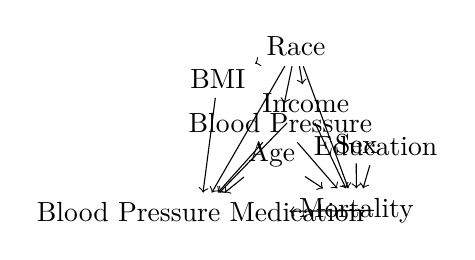
\begin{tikzpicture}
\node (v0) at (-1.62,-1.53) {Blood Pressure Medication};
\node (v1) at (-0.606,-0.394) {Blood Pressure};
\node (v2) at (-0.714,-0.797) {Age};
\node (v3) at (-1.40,0.165) {BMI};
\node (v4) at (0.604,-0.687) {Education};
\node (v5) at (-0.282,-0.151) {Income};
\node (v6) at (0.361,-1.51) {Mortality};
\node (v7) at (-0.406,0.572) {Race};
\node (v8) at (0.357,-0.659) {Sex};
\draw [->] (v0) edge (v6);
\draw [->] (v1) edge (v0);
\draw [->] (v1) edge (v6);
\draw [->] (v2) edge (v0);
\draw [->] (v2) edge (v6);
\draw [->] (v3) edge (v0);
\draw [->] (v4) edge (v6);
\draw [->] (v5) edge (v0);
\draw [->] (v5) edge (v6);
\draw [->] (v7) edge (v0);
\draw [->] (v7) edge (v1);
\draw [->] (v7) edge (v3);
\draw [->] (v7) edge (v5);
\draw [->] (v7) edge (v6);
\draw [->] (v8) edge (v6);
\end{tikzpicture}

\hypertarget{ltmle-estimation-1}{%
\subsection{LTMLE Estimation}\label{ltmle-estimation-1}}

Use the \texttt{ltmle} package for this section. First fit a ``naive
model'' that \textbf{does not} control for the time-dependent
confounding. Then run a LTMLE model that does control for any time
dependent confounding. Follow the same steps as in the TMLE section. Do
you see a difference between the two estimates?

\begin{Shaded}
\begin{Highlighting}[]
\DocumentationTok{\#\# Naive Model (no time{-}dependent confounding) estimate}

\DocumentationTok{\#\# LTMLE estimate}
\end{Highlighting}
\end{Shaded}

\hypertarget{discussion-questions-2}{%
\subsection{Discussion Questions}\label{discussion-questions-2}}

\begin{enumerate}
    \item What sorts of time-dependent confounding should we be especially worried about? For instance, would we be concerned about a running variable for age the same way we might be concerned about blood pressure measured at two different times?
\end{enumerate}

\end{document}
